%%%%%%%%%%%%%%%%%%%%%%%%%%%%%%%%%%%%%%%%%%%%%%%%%%%%%%%%%%%%
% Theory book for guitarists
%
%%%%%%%%%%%%%%%%%%%%%%%%%%%%%%%%%%%%%%%%%%%%%%%%%%%%%%%%%%%%

%----------------------------------------------------------------------------------------
%	PACKAGES AND DOCUMENT CONFIGURATIONS
%----------------------------------------------------------------------------------------

\documentclass{article}

% Latex packages
\usepackage{parskip}
\usepackage[shortlabels]{enumitem}
\usepackage{graphicx} % Required for the inclusion of images
\usepackage{amsmath,amssymb} % Required for some math elements
\usepackage{caption}
\usepackage{subcaption}
\usepackage{hyperref}
\setlength\parindent{0pt} % Removes all indentation from paragraphs
\usepackage{booktabs}
\usepackage{changepage}
\usepackage{multirow}
\usepackage{pgfplots} % Include package for TikZ and PGF plot
\usepackage{anyfontsize} % enable to change the font size manually
\usepackage{makecell}%
\usetikzlibrary{shapes.geometric}
\tikzset{
  dot/.style = {circle, fill, minimum size=#1,
                inner sep=0pt, outer sep=0pt},
  dot/.default = 6pt
}


\renewcommand{\labelenumi}{\alph{enumi}.} % Make numbering in the enumerate environment by letter rather than number (e.g. section 6)

%% Recherche des images dans les répertoires.
\graphicspath{{./figures/}{./dia/}{./gnuplot/}}

\title{ Music theory for guitar nerds  } % Title
\author{ Jean-Hughes \textsc{Fournier L.} } % Author name
\date{\today} % Date for the report

\begin{titlepage}
    \centering
	\vspace*{-3cm}
	\hspace*{-5cm}
    \includegraphics[width=22cm]{cover_picture/cover1.jpeg} % scale as needed
    \vfill
\end{titlepage}



% Plan:
%
% 1. Intervals (Why intervals are consonant or dissonant?, Harmonic series, harmonic entropy, battement)
%      1.1 Harmonic series
%      1.2 Consonance and dissonance
% 2. Scales    (Major scale, minor scales, pattern on fretboard)
% 3. Chords    (Triad, tetrad, pentad)
%  3.1 Chord progressions (Circle of fifths)
% 4. Modes     (Table of modes)
% 5. Arpeggios



%***********************************************************************************************************************************************
\begin{document}

\maketitle % Insert the title, author and date
\newpage
\tableofcontents
\newpage

\begin{itemize}
	\item Gives the recipe not just examples
	\item If you give a man a fish, you feed him for a day. If you teach a man to fish, you feed him for a lifetime
\end{itemize}

%%%%%%%%%%%%%%%%%%%%%%%%%%%%%%%%%%%%%%%%%%%%%%%%%%%%%%%%%%%%%%%%%%%%%%%
\section{Intervals: where do notes come from?}
%%%%%%%%%%%%%%%%%%%%%%%%%%%%%%%%%%%%%%%%%%%%%%%%%%%%%%%%%%%%%%%%%%%%%%%

%Names of the interval comes from the diatonic scale. In C major scale (C-D-E-F-G-A-B-C) that scale G$\#$ is the augmented 5. In C minor scale (C-D-Eb-F-G-Ab-Bb) G$\#$ is the minor sixth.

\subsection{Harmonic series}

% Figure
\begin{figure}[h!]
	\centering
%	\hspace*{0cm}
	\scalebox{1}{\input{figures/serie_harmonique.tex}}
	\caption{The harmonic series}
	\label{fig:serie_harmonique}
\end{figure}

% Table
\input{tableaux/harmoniques}


 Table
 Source: https://hellomusictheory.com/learn/intervals/
\begin{table*}[!h]
	\caption{Intervals chart in relation to C note. Minor (m or ``-''), major (M or ``maj''), augmented (A or ``aug'' or ``$\#$'' or ``$+$'') and diminished (d or ``dim'' or ``b''). }
	\centering
	\begin{adjustwidth}{-2cm}{}
	\begin{tabular}{clclcl}
		\hline 
		\textbf{Semitones} & \textbf{Name} & \textbf{Notation} & \textbf{Songs}  \\
		\hline
		0 & Perfect unison            & P1 & -   \\
		\hline
		1 & Minor second              & m2 & JAWS theme \\
		2 & Major second              & M2 & \textbf{Frè-re} Jacques  \\
		\hline
		3 & Minor third               & m3 & Iron Man by Black Sabbath\\
		4 & Major third               & M3 & "\textbf{Oh-When} the Saints" \\
		\hline
		5 & Perfect fourth            & P4 & Here Comes the Bride (Wedding song) \\
		\hline
		6 & Triton                    & T  & "\textbf{The - Simp}-sons" \\ 
		\hline
		7 & Perfect fifth             & P5 &  "\textbf{Twinkle - Twinkle} Little Star"   \\
		\hline
		8 & Minor sixth               & m6 &  The Entertainer \\
		9 & Major sixth               & M6 &  Jingle Bells ("\textbf{Dash-ing} through the snow")   \\
		\hline
		10 & Minor seventh            & m7 &  Theme song Star Trek : The Original Series\\
		11 & Major seventh            & M7 &  Take On Me ("Take-on")  \\
		\hline
		12 & Perfect octave           & P8 &  "\textbf{Some-where} over the rainbow" \\
		\hline
		13 & Minor ninth              & m9 &  - \\
		14 & Major ninth              & M9 &  - \\
		\hline
		16 & Diminished eleventh      & d11 & - \\
		17 & Perfect eleventh         & P11 & - \\
		18 & Augmented eleventh       & A11 & - \\
		\hline
		20 & Minor thirteenth         & m13 & - \\
		21 & Major thirteenth         & M13 & - \\
		\hline
	\end{tabular}
	\end{adjustwidth}
	\label{tab: }
\end{table*}


% ****************************************************************************
\subsection{Consonance and dissonance}

% Figure
\begin{figure}[h!]
	\centering
	\hspace*{0cm}
	\includegraphics[scale=0.03, trim= {0cm 0cm 0cm 0cm}, clip]{Harmonic_entropy.png}
	\caption{Harmonic entropy}
	\label{fig}
\end{figure}

% Figure
\begin{figure}[h!]
	\centering
	\hspace*{0cm}
	\includegraphics[scale=0.5, trim= {0cm 0cm 0cm 0cm}, clip]{battement/main.pdf}
%	\scalebox{0.3}{\documentclass{standalone}
\usepackage{pgfplots} % Include package for TikZ and PGF plot
\usepackage{anyfontsize} % enable to change the font size manually 
\usepackage{makecell}%
\usetikzlibrary{shapes.geometric}
\tikzset{
dot/.style = {circle, fill, minimum size=#1,
              inner sep=0pt, outer sep=0pt},
dot/.default = 6pt % size of the circle diameter 
}
 \renewcommand{\familydefault}{\sfdefault}

\begin{document}
\begin{tikzpicture}[scale=1]
	\def \R{10cm}
	
	
	\draw[black, thick] (0,0) circle (\R); 
	\draw[black, thick] (0,0) circle (2*\R/3); 
	
	
	\node[] at (0,8cm) {{\large C}};
	
	%\fill[black, line width=2] (0.0,-0.4) rectangle (20*\fret,4.4);
	%\draw[color=black!50!white, thick]  (0, 0)   -- (0,5*\h); 
	
	
\end{tikzpicture}
\end{document}}
	\caption{Beat tone}
	\label{fig}
\end{figure}


%%%%%%%%%%%%%%%%%%%%%%%%%%%%%%%%%%%%%%%%%%%%%%%%%%%%%%%%%%%%%%%%%%%%%%%
% Interval of notes create scales
\newpage
\section{Scales}
%%%%%%%%%%%%%%%%%%%%%%%%%%%%%%%%%%%%%%%%%%%%%%%%%%%%%%%%%%%%%%%%%%%%%%%

% Table
\input{tableaux/gammes.tex}

\newpage
\subsection{Major scale}
Modes ranked by brightness: Super-locrian, locrian, phrygian, aeolian, dorian, mixolydian, major, lydian, lydian augmented

\begin{itemize}
	\item Major scales and the modes (and all modes)
	\item Pentatonic scale (Major, Egyptian, Man Gong, Ritusen)
	\item Minor scale (natural, harmonic, melodic)
	\item Phrygian dominant (hijaz) (I-bII-iiidim-iv-vdim-bVI+-bvii)  Ex: Come out and Play The Offsprings
\end{itemize}

% Figure
\begin{figure}[h!]
	\centering
	\hspace*{-2cm}
%	\includegraphics[scale=0.55, trim= {0cm 0cm 0cm 0cm}, clip]{gamme_majeure_manche/main.pdf}
	\scalebox{0.5}{\input{figures/gamme_majeure_manche.tex}}
	\caption{G Major scale on the fretboard}
	\label{fig:gamme_majeure_manche}
\end{figure}

\newpage
\subsection{Pentatonic scale}
% Figure
\begin{figure}[h!]
	\centering
	\hspace*{-2cm}
%	\includegraphics[scale=0.55, trim= {0cm 0cm 0cm 0cm}, clip]{gamme_penta_manche/main.pdf}
	\scalebox{0.5}{\input{figures/gamme_penta_manche.tex}}
	\caption{Pattern of pentatonic scales}
	\label{fig:gammme_penta_manche}
\end{figure}

\newpage
\subsection{Blues}


% Table
\begin{table*}[!h]
	\caption{Blues scales (relative to the major scale)}
	\centering
	%\begin{adjustwidth}{0cm}{}
	\begin{tabular}{l|cccccccc}
		Scale name  & \multicolumn{8}{c}{Formula} \\
		\hline \hline \vspace{-0.4cm} \\
		Blues Major   & 1 & 2  & \textcolor{red}{b3} & 3  &   -   & 5  & 6  &  -  \\
		Blues minor   & 1 &  - & b3 & 4  & \textcolor{red}{b5} &  5  & - &  b7 \\
	\end{tabular}
	\label{tab: }
	%\end{adjustwidth}
\end{table*}

% Table
% % Jake Lizzio
\begin{table*}[!h]
	\caption{Basic 12 bar major blues}
	\centering
	\begin{tabular}{| c | c | c | c |}
		\hline
		\phantom{x}I7\phantom{x} & \phantom{x}I7\phantom{x} & \phantom{x}I7\phantom{x} & \phantom{x}I7\phantom{x}  \\
		\hline
		\phantom{x}IV7\phantom{x} & \phantom{x}IV7\phantom{x} & \phantom{x}I7\phantom{x} & \phantom{x}I7\phantom{x}  \\
		\hline
		\phantom{x}V7\phantom{x} & \phantom{x}IV7\phantom{x} & \phantom{x}I7\phantom{x} & \phantom{x}I7\phantom{x}  \\
		\hline
	\end{tabular}
	\label{tab: }
\end{table*}

\begin{table*}[!h]
	\caption{Basic 12 bar minor blues}
	\centering
	\begin{tabular}{| c | c | c | c |}
		\hline
		\phantom{x}i7\phantom{x} & \phantom{x}i7\phantom{x} & \phantom{x}i7\phantom{x} & \phantom{x}i7\phantom{x}  \\
		\hline
		\phantom{x}iv7\phantom{x} & \phantom{x}iv7\phantom{x} & \phantom{x}i7\phantom{x} & \phantom{x}i7\phantom{x}  \\
		\hline
		\phantom{x}v7 or V7\phantom{x} & \phantom{x}iv7\phantom{x} & \phantom{x}i7\phantom{x} & \phantom{x}V7\phantom{x}  \\
		\hline
	\end{tabular}
	\label{tab: }
\end{table*}

\begin{table*}[!h]
	\caption{Basic 12 bar major blues with a \textit{quick change} and \textit{turnaroun}d}
	\centering
	\begin{tabular}{| c | c | c | c |}
		\hline
		\phantom{x}I7\phantom{x} & \phantom{x}\textbf{IV7}\phantom{x} & \phantom{x}I7\phantom{x} & \phantom{x}I7\phantom{x}  \\
		\hline
		\phantom{x}IV7\phantom{x} & \phantom{x}IV7\phantom{x} & \phantom{x}I7\phantom{x} & \phantom{x}I7\phantom{x}  \\
		\hline
		\phantom{x}V7\phantom{x} & \phantom{x}IV7\phantom{x} & \phantom{x}I7 - \textbf{vi7} & \textbf{ii7} - V7\phantom{x}  \\
		\hline
	\end{tabular}
	\label{tab: }
\end{table*}

% Figure
\begin{figure}[h!]
	\centering
	\hspace*{-1cm}
	\scalebox{0.7}{\input{figures/blues_penta_mineur.tex}}
%	\vspace{10cm}
	\hspace*{-1cm}
	\scalebox{0.7}{
\renewcommand{\familydefault}{\sfdefault}

%\begin{document}
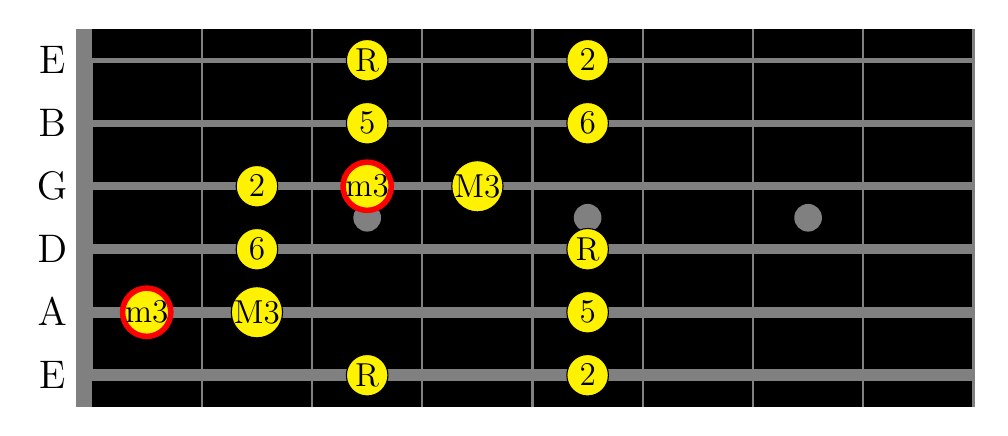
\begin{tikzpicture}[scale=1]
	\def \h{0.8}
	\def \fret{1.4} % 1.6
	\def \L{ 8*\fret }	
	\def \dot_size{5pt}
	\def \circ_size{15pt}
	
	\fill[black, line width=2] (0.0,-0.4) rectangle (8*\fret,4.4);
	\fill[black!50!white, line width=2] (-0.2,-0.4) rectangle (0,4.4);
	
	% Strings
	\draw[color=black!50!white, line width=2.0]  (-0.1, 5*\h) -- (\L,5*\h); % E
	\draw[color=black!50!white, line width=2.5]  (-0.1, 4*\h) -- (\L,4*\h); % B
	\draw[color=black!50!white, line width=3.0]  (-0.1, 3*\h) -- (\L,3*\h); % G
	\draw[color=black!50!white, line width=3.5]  (-0.1, 2*\h) -- (\L,2*\h); % D
	\draw[color=black!50!white, line width=4.0]  (-0.1, 1*\h) -- (\L,1*\h); % A
	\draw[color=black!50!white, line width=4.5]  (-0.1, 0*\h) -- (\L,0*\h); % E
	
	% Frets 0
	\draw[color=black!50!white, thick]  (-0.1, 0) -- (-0.1,5*\h); 
	\draw[color=black!50!white, thick]  (0, 0)   -- (0,5*\h); 
	
	% Fret 1-15
	\draw[color=black!50!white, thick]  (\fret,   -0.4)   -- (\fret,4.4);   
	\draw[color=black!50!white, thick]  (2*\fret, -0.4) -- (2*\fret,4.4); 
	\draw[color=black!50!white, thick]  (3*\fret, -0.4) -- (3*\fret,4.4); 
	\draw[color=black!50!white, thick]  (4*\fret, -0.4) -- (4*\fret,4.4); 
	\draw[color=black!50!white, thick]  (5*\fret, -0.4) -- (5*\fret,4.4); 
	\draw[color=black!50!white, thick]  (6*\fret, -0.4) -- (6*\fret,4.4); 
	\draw[color=black!50!white, thick]  (7*\fret, -0.4) -- (7*\fret,4.4); 
	\draw[color=black!50!white, thick]  (8*\fret, -0.4) -- (8*\fret,4.4);
	
	% Dots
	\fill[black!50!white] (2.5*\fret,2.5*\h) circle (\dot_size); % fret 3
	\fill[black!50!white] (4.5*\fret,2.5*\h) circle (\dot_size); % fret 5
	\fill[black!50!white] (6.5*\fret,2.5*\h) circle (\dot_size); % fret 7
	
	% String names
	\draw[black] (-0.5,5*\h) node { {\Large E} };
	\draw[black] (-0.5,4*\h) node { {\Large B} };
	\draw[black] (-0.5,3*\h) node { {\Large G} };
	\draw[black] (-0.5,2*\h) node { {\Large D} };
	\draw[black] (-0.5,1*\h) node { {\Large A} };
	\draw[black] (-0.5,0*\h) node { {\Large E} };
	
	% Major scale (fret 1-5)
	\node[dot=\circ_size, fill=yellow,draw] at (2.5*\fret,0) {{\large \textcolor{black}{R}}};    % Root
	\node[dot=\circ_size, fill=yellow, draw] at (4.5*\fret,0) {{\large 2}};
	\node[dot=\circ_size, fill=yellow,draw] at (1.5*\fret,1*\h) {{\large M3}};
	\node[dot=\circ_size, draw=red, line width=2, fill=yellow, draw] at (0.5*\fret,1*\h) {{\large m3}};
	\node[dot=\circ_size, fill=yellow,draw] at (4.5*\fret,1*\h) {{\large 5}};
	\node[dot=\circ_size, fill=yellow,draw] at (1.5*\fret,2*\h) {{\large 6}};
	\node[dot=\circ_size, fill=yellow,draw] at (4.5*\fret,2*\h) {{\large R}}; % Root
	\node[dot=\circ_size, fill=yellow,draw] at (1.5*\fret,3*\h) {{\large 2}};
	\node[dot=\circ_size, fill=yellow,draw] at (3.5*\fret,3*\h) {{\large M3}};
	\node[dot=\circ_size, draw=red, line width=2, fill=yellow, draw] at (2.5*\fret,3*\h) {{\large m3}};
	\node[dot=\circ_size, fill=yellow,draw] at (2.5*\fret,4*\h) {{\large 5}};
	\node[dot=\circ_size, fill=yellow,draw] at (4.5*\fret,4*\h) {{\large 6}};
	\node[dot=\circ_size, fill=yellow,draw] at (2.5*\fret,5*\h) {{\large R}};
	\node[dot=\circ_size, fill=yellow,draw] at (4.5*\fret,5*\h) {{\large 2}};

	
\end{tikzpicture}
%\end{document}









}
	\hspace*{-1cm}
	\scalebox{0.7}{\input{figures/blues_penta.tex}}
	\caption{(a) Minor pentatonic scale with blue note (b5). (b) Major pentatonic scale. (c) Blues scale  }
	\label{fig:blues_penta_mineur}
\end{figure}

%%%%%%%%%%%%%%%%%%%%%%%%%%%%%%%%%%%%%%%%%%%%%%%%%%%%%%%%%%%%%%%%%%
% Construction of chords superimposing 3rds on a scale
\newpage
\section{Chords}
%%%%%%%%%%%%%%%%%%%%%%%%%%%%%%%%%%%%%%%%%%%%%%%%%%%%%%%%%%%%%%%%%%%%%%%

\begin{itemize}
	\item Tonic: I, iii, vi
	\item Pre-dominant: IV, ii
	\item Dominant: V, vii$^\circ$
\end{itemize}


\begin{itemize}
	\item ``Sus'' chords: chord without third
	\item ``sus9'' will often replace the dominant 7th chord
\end{itemize}

%%%%%%%%%%%%%%%%%%%%%%%%%%%%%%%%%%%%%%%%%%%%%%%%%%%%%%%%%%%%%%%%%%%%%%%%%%%%%%%%%%%%%%%%%%%%%%%%%%%%%%%%%
\newpage
\subsection{Formation of chords}

% Table
% Source: 1997 - Vaillot Méthode Jazz
% Tetrad: https://www.beyondmusictheory.org/chord-formations-triads-and-tetrads/
% Nom de acccords Jake lizzio
\begin{table*}[!h]
	\centering
	\caption{Construction of chords (notation is relative to the major scale)}
	\begin{tabular}{clcccccc}
		\hline \vspace{-0.2cm} \\
		$\#$ notes & Chords & & & & & &\\
		\hline \vspace{-0.2cm} \\
		\multirow{6}{*}{triad} & -        & 1 & M3 & 5 &  -  & -  & -\\
		                       & m        & 1 & m3 & 5 &  -  & -  & -\\
		                       & dim or $^\circ$  & 1 & m3 & b5  &  -  & -  & -\\
		                       & aug or $^\#$5 & 1 & m3 & $^\#$5 &  -  & -  & -\\
		                       & sus2     & 1 & M2  & 5     &  -  & -  & -\\
		                       & sus4     & 1 & 4   & 5     &  -  & -  & -\\
		\hline
		\multirow{13}{*}{tetrad}& 7        & 1 & M3  & 5 & m7  & -  & -\\
		                       & $\Delta$  & 1 & M3  & 5 & M7  & -  & -\\
		                       & m$^7$     & 1 & m3  & 5 & m7  & -  & -\\
		                       & m$^\Delta$& 1 & m3  & 5 & M7  & -  & -\\
		                       & m$^{7\textrm{b}5}$ or $\varnothing$& 1 & m3  & b5 & m7  & -  & -\\
		                       & $^{\circ 7}$   & 1 & m3  & b5 & b7 & -  & -\\
                               & 6        & 1 & M3  & 5 & 6   & -  & -\\
                               & m6       & 1 & m3  & 5 & 6   & -  & -\\
		                       & m6(9)    & 1 & m3  & 6 & M9  & -  & -\\
		                       & 6(9)     & 1 & M3  & 6 & M9  & -  & -\\
		                       & 7sus4    & 1 & 4   & 5 & m7  & -  & -\\
		                       & add2     & 1 & M2  & M3& 5   & -  & -\\
		                       & add9     & 1 & M3  & 5 & M9  & -  & -\\
		\hline
		\multirow{6}{*}{pentad}& 7(b9)      & 1 & M3  & 5 & m7  & m9  & -\\
	                           & $\Delta^9$ & 1 & M3  & 5 & M7  & M9  & -\\
		                       & 9          & 1 & M3  & 5 & m7  & M9  & -\\
		                       & m9         & 1 & m3  & 5 & m7  & M9  & -\\
		                       & sus9       & 1 & 4   & 5 & m7  & M9  & -\\
		                       & 11         & 1 & 5   & m7& M9  & 11  & -\\ % The 3 is omitted to avoid the dissonace between 3-11.
		\hline
		\multirow{2}{*}{hexad} & 7(13)      & 1 & M3  & 5 & m7  & M9  & M13\\ % the 11 is omited to avoid the dissonance between 3-11.
		                       & 7(b9,13)   & 1 & M3  & 5 & m7  & m9  & M13\\
		\hline \vspace{-0.2cm}
	\end{tabular}
	\label{tab: }
\end{table*}

- Accords: 7, m7, maj7, m7b5 (root sur corde E, A, D)

\newpage
\subsection{Harmonizing the major scale}
% Table

\begin{table*}[!h]
	\caption{Harmonization of scales (relative to major scale)}
	\begin{adjustwidth}{0cm}{}
	\begin{tabular}{r|ccc cccc}
		\hline \vspace{-0.4cm} \\
		& 1 & 2 & 3 & 4 & 5 & 6 & 7\\
		\hline \vspace{-0.2cm} \\
		Major  & I$^\Delta$ & ii$^{-7}$ & iii$^{-7 \phantom{\textrm{aug}}$ & IV$^\Delta$ & V$^7$ & vi$^{-7}$ & vii$^{\varnothing}$ \\
		\hline \vspace{-0.2cm} \\
		Natural minor  & i$^{-7}$ & ii$^{\varnothing}$ & bIII$^{\Delta \phantom{\textrm{aug}}}$ & iv$^{-7}$ & v$^{-7}$ & bVI$^{\Delta}$ & bVII$^{7}$ \\
		\hline \vspace{-0.2cm} \\
		Harmonic minor & i$^{\Delta}$ & ii$^{\varnothing}$ & bIII$^{\Delta, \textrm{aug}}$ & iv$^{-7}$ & V$^7$ & bVI$^{\Delta}$ & vii$^{\circ 7}$ \\
		\hline \vspace{-0.2cm} \\
		Melodic minor & i$^{\Delta}$ & ii$^{-7}$ & bIII$^{\Delta, \textrm{aug}}$ & IV$^7$ & V$^7$ & vi$^{\varnothing}$ & vii$^{\varnothing}$ \\
		\hline \vspace{-0.2cm} \\
		Dorian        & i$^{-7}$ & ii$^{-7}$ & bIII$^{\Delta, \phantom{\textrm{aug}}}$ & IV$^{7}$ & v$^{-7}$ & vi$^{\varnothing}$ & bVII$^{\Delta}$ \\
		\hline
	\end{tabular}
	\label{tab: }
	\end{adjustwidth}
\end{table*}

% Table

\begin{table*}[!h]
	\caption{Table of modes }
	\begin{adjustwidth}{-2.3cm}{}
	\begin{tabular}{lccc cccc}
		\hline \vspace{-0.2cm} \\
		Mode name & Ionian & Dorian & Phrygian & Lydian & Mixolydian & Aeolian & Locrian\\
		\hline \vspace{-0.2cm} \\
		Diatonic chords & I & ii$ & iii  & IV & V & vi & vii$^{\circ}$ \\
		Diatonic seventh & $\Delta$7 & $^{-}$7 & $^{-}$7  & $\Delta$7 & 7 & $^{-}$7 & $\varnothing$ \\
		Alternative naming & maj7 & m7 & m7 & maj7 & 7 & m7 & m7b5\\
		%Diatonic seventh  & $\Delta$7 & $^{-}$7 & $^{-}$7 & $\Delta$7 & 7 & $^{-}$7 & $\varnothing$ \\
		\hline \vspace{-0.2cm} \\
		{\scriptsize $\# \# \# \# \# \#$} & F$^\#$ & G$^\#$ & A$^\#$ & B & C$^\#$ & D$^\#$ & E$^\#$ \\
		{\scriptsize $\# \# \# \# \#$}    & B & C$^\#$ & D$^\#$ & E & F$^\#$ & G$^\#$ & A$^\#$\\
		{\scriptsize $\# \# \# \#$}       & E & F$^\#$ & G$^\#$ & A & B & C$^\#$ & D$^\#$\\
		{\scriptsize $\# \# \#$}          & A & B & C$^\#$ & D & E & F$^\#$ & G$^\#$\\
		{\scriptsize $\# \#$}             & D & E & F$^\#$ & G & A & B & C$^\#$\\
		{\scriptsize $\#$}                & G & A & B & C  & D & E & F$^\#$\\
		{\scriptsize -}                   & \textbf{C} & \textbf{D} & \textbf{E} & \textbf{F} & \textbf{G} & \textbf{A} & \textbf{B}\\
		{\scriptsize b}                   & F  & G  & A  & B$^\textrm{b}$ & C  & D  & E\\
		{\scriptsize bb}                  & B$^\textrm{b}$ & C     & D     & E$^\textrm{b}$ & F     & G     & A\\
		{\scriptsize bbb}                 & E$^\textrm{b}$ & F     & G     & A$^\textrm{b}$ & B$^\textrm{b}$ & C     & D\\
		{\scriptsize bbbb}                & A$^\textrm{b}$ & B$^\textrm{b}$ & C     & D$^\textrm{b}$ & E$^\textrm{b}$ & F     & G\\
		{\scriptsize bbbbb}               & D$^\textrm{b}$ & E$^\textrm{b}$ & F     & G$^\textrm{b}$ & A$^\textrm{b}$ & B$^\textrm{b}$ & C\\
		{\scriptsize bbbbbb}              & G$^\textrm{b}$ & A$^\textrm{b}$ & B$^\textrm{b}$ & C$^\textrm{b}$ & D$^\textrm{b}$ & E$^\textrm{b}$ & F\\
		\hline
		\hline \vspace{-0.2cm}
	\end{tabular}
	\label{tab: }
	\end{adjustwidth}
\end{table*}

\newpage
\subsection{Chord progression and example}

% Table
% Source: 1997 - Vaillot Méthode Jazz

\begin{table*}[!h]
	\centering
	\caption{Famous chord progressions}
	\begin{adjustwidth}{-3cm}{}
	\begin{tabular}{p{5.0cm}p{5.5cm}p{7cm}}
		\hline \vspace{-0.2cm} \\
	    Name & Progression & Example\\
		\hline \vspace{-0.2cm} \\
		Pop major (punk)      & $\textrm{I}-\textrm{V}-\textrm{vi}-\textrm{IV}$ & Dammit, Let it be, Country Road \\
		Anatol (turnaround)   & $\textrm{I}^{\Delta}-\textrm{vi}^7-\textrm{ii}^7-\textrm{V}^7$ & Blue Moon \\
		50s progression       & $\textrm{I}-\textrm{vi}-\textrm{IV}-\textrm{V}$ & Every Breath You Take, Crocodile Rock\\
		Ragtime               &$\textrm{I}-\textrm{VI}^7-\textrm{II}^{7}-\textrm{V}^{7}$ & I want to be like you (Disney) \\
		Jazz (ii-V-I)         & $\textrm{ii}^{7}-\textrm{V}^7-\textrm{I}^{\Delta}$ & Autumn leaves\\
		Blues/Rock (Major)    & $\textrm{I}^7-\textrm{IV}^7-\textrm{V}^7-\textrm{I}^7$ & Johnny B. Goode\\

	    Mixo vamp (mixo)      & $\textrm{I}-\textrm{bVII}-\textrm{IV}-\textrm{I}$ & Hey Jude, Sweet home Alabama \\
	    Japanese ``Royal road'' & $\textrm{IV}^\Delta-\textrm{V}^7-\textrm{iii}^7-\textrm{vi}^7-$ {\footnotesize $(\textrm{ii}^7-\textrm{V}^7-\textrm{I}^{\Delta})$} & Shogo theme, anime \\
	    ``Storyteller''       & $\textrm{I}-\textrm{IV}-\textrm{vi}-\textrm{V}$ & \\
	    Creep chord            & I$\,-\,$III$\,-\,$IV$\,-\,$iv &  Creep, Space Oddity \\
		Pop minor             & $\textrm{i}-\textrm{bVI}-\textrm{bIII}-\textrm{bVII}$ & Save Tonight, Africa Toto \\
	    Aeolian vamp          & $\textrm{i}-\textrm{bVII}-\textrm{bVI}-\textrm{bVII}$  & Stairway to Heaven, All Iron Maiden \vspace{-0.8cm}  \\
		Minor progression 01    & $\textrm{i}-\textrm{i}-\textrm{bVI}-\textrm{V}$ & Sweet Dreams \\
	    Minor progression 02    & $\textrm{i}-\textrm{bVI}-\textrm{bIII}-\textrm{bVII}$ &  \\
	    Minor progression 03    & $\textrm{i}-\textrm{bVI}-\textrm{iv}-\textrm{bVII}$ & Final countdown\\
	    Minor progression 04    & $\textrm{i}-\textrm{bIII}-\textrm{bVII}-\textrm{iv}$ & Boulevard of Broken Dreams\\
	    Andalusian	(phrygian)& $\textrm{i}-\textrm{bVII}-\textrm{bVI}-\textrm{V}^7$ & Happy Together The Turtles\\
	    Blues/Rock (minor)      & $\textrm{i}^7-\textrm{iv}^7-\textrm{V}^7-\textrm{i}^7$ & Minor swing\\
	    Anime                   & $\textrm{bVI}-\textrm{bVII}-\textrm{i}$   &             \\
		Neapolitan              & i$\,-\,$bII$^6\,-\,$V$\,-\,$i &  Classic \\
		\hline \vspace{-0.2cm} \\
	\end{tabular}
	\end{adjustwidth}
	\label{tab:}
\end{table*}

%%%%%%%%%%%%%%%%%%%%%%%%%%%%%%%%%%%%%%%%%%%%%%%%%%%%%%%%%%%%%%%%%%%%%%%%%%%%%%%%%%%%%%%%%%%%%%%%%%%%%%%%%
\newpage
\subsection{Chord inversions}

- Accords: 7, m7, maj7, m7b5 (root: E, A, D)

% Figure
\begin{figure}[h!]
	\centering
	\hspace*{-2.2cm}
	\includegraphics[scale=0.7, trim= {0cm 0cm 0cm 0cm}, clip]{figures/chord-inversions/maj7.pdf}
	\hspace*{-2.2cm}
	\includegraphics[scale=0.7, trim= {0cm 0cm 0cm 0cm}, clip]{figures/chord-inversions/Dominant7.pdf}
	\hspace*{-2.2cm}
	\includegraphics[scale=0.7, trim= {0cm 0cm 0cm 0cm}, clip]{figures/chord-inversions/m7.pdf}
	\caption{(a) maj7 chords. (b) Dominnt 7 chords. (c) m7 chords  }
	\label{fig}
\end{figure}

%%%%%%%%%%%%%%%%%%%%%%%%%%%%%%%%%%%%%%%%%%%%%%%%%%%%%%%%%%%%%%%%%%%%%%%%%%%%%%%%%%%%%%%%%%%%%%%%%%%%%%%%%


Concepts:
\begin{itemize}
	\item Borrowed chord: chord that is not built from the scale of the tonic. Examples:
	\begin{itemize}
		\item ``Picardy third'': a progression with an ending major triad instead of an expected minor triad to create an impression of resolution.
		\item Use the bVII
	\end{itemize}
	\item Transistion Chords:
	\begin{itemize}
		\item Secondary dominant chord (tonicization) (V/x): using the fifth of a chord (even if it's not a diatonic chord) in order to feel a ``resolution'' on this chord.
		\item Tritone substitution (Vsub/x or bV7/V): Approach any target chord with a diminished 7 chord a semitone above.
		\item Backdoor [ii V]. Approach the tonic with iv7 - bVII7 - I.
		\item Modulation (Rick Beato):
		\begin{itemize}
			\item Diatonic common chord (``close'' keys have many chords in common that can be used to modulate from a key to another. Common chords are called pivot chords)
			\item Chromatic pivot chord
			\item Enharmonic dominant
			\item Deceptive
			\item Enharmonic Dim7
			\item Dim7 to Dom7 (lower the root of the dim7 chord to create a dominant chord that leads to a new tonic)
			\item Chromatic Mediant
			\item Common tone (Pivot note)
			\item Direct or Linear (Abrupt change of key without preparation to ``lift'' the song)
			\item Chain Modulation ()
			\item Parallel modulation (Modulation of the mode but keep the same root ex: C to Cm)
		\end{itemize}
	\end{itemize}
\end{itemize}


% Figure
\begin{figure}[h!]
	\centering
	\hspace*{-1cm}
	\includegraphics[scale=0.3, trim= {0cm 0cm 0cm 0cm}, clip]{Circle_5th.png}
	\caption{ }
	\label{fig}
\end{figure}

\begin{itemize}
	\item Substitution tritonique
	\item Substitution diatonique
\end{itemize}


%%%%%%%%%%%%%%%%%%%%%%%%%%%%%%%%%%%%%%%%%%%%%%%%%%%%%%%%%%%%%%%%%%
\newpage
\section{Arpeggios}


% Figure
\begin{table}[!h]
	\hspace*{-4.2cm}
	\scalebox{0.52}{\input{figures/arpeges/dom7/dom7_pos1.tex}}
	\hspace*{-0cm}
	\scalebox{0.52}{\input{figures/arpeges/m7/m7_pos1.tex}}

	\hspace*{-4.2cm}
	\scalebox{0.52}{\input{figures/arpeges/dom7/dom7_pos2.tex}}
	\hspace*{-0cm}
	\scalebox{0.52}{\input{figures/arpeges/m7/m7_pos2.tex}}

	\hspace*{-4.2cm}
	\scalebox{0.52}{\input{figures/arpeges/dom7/dom7_pos3.tex}}
	\hspace*{-0cm}
	\scalebox{0.52}{\input{figures/arpeges/m7/m7_pos3.tex}}

	\hspace*{-4.2cm}
	\scalebox{0.52}{\input{figures/arpeges/dom7/dom7_pos4.tex}}
	\hspace*{-0cm}
	\scalebox{0.52}{\input{figures/arpeges/m7/m7_pos4.tex}}

	\hspace*{-4.2cm}
	\scalebox{0.52}{\input{figures/arpeges/dom7/dom7_pos5.tex}}
	\hspace*{-0cm}
	\scalebox{0.52}{

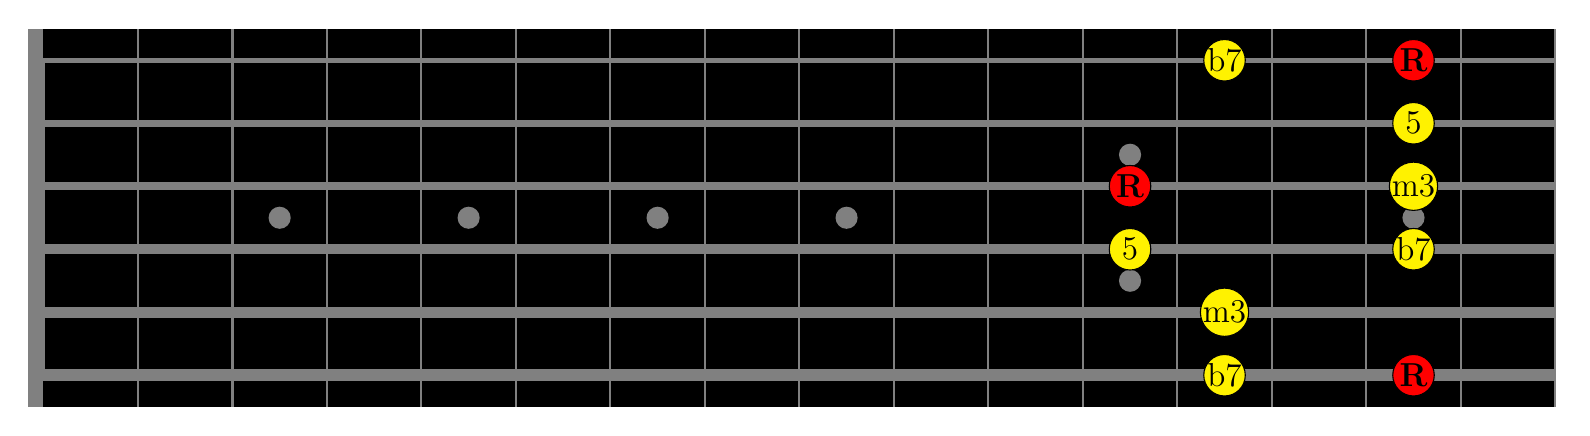
\begin{tikzpicture}[scale=1]
	\def \h{0.8}
	\def \fret{1.2} % 1.6
	\def \L{ 16*\fret }
	\def \dot_size{4pt}
	\def \circ_size{15pt}

	\fill[black, line width=2] (0.0,-0.4) rectangle (16*\fret,4.4);
	\fill[black!50!white, line width=2] (-0.2,-0.4) rectangle (0,4.4);

	% Strings
	\draw[color=black!50!white, line width=2.0]  (-0.1, 5*\h) -- (\L,5*\h); % E
	\draw[color=black!50!white, line width=2.5]  (-0.1, 4*\h) -- (\L,4*\h); % B
	\draw[color=black!50!white, line width=3.0]  (-0.1, 3*\h) -- (\L,3*\h); % G
	\draw[color=black!50!white, line width=3.5]  (-0.1, 2*\h) -- (\L,2*\h); % D
	\draw[color=black!50!white, line width=4.0]  (-0.1, 1*\h) -- (\L,1*\h); % A
	\draw[color=black!50!white, line width=4.5]  (-0.1, 0*\h) -- (\L,0*\h); % E

	% Frets 0
	\draw[color=black!50!white, thick]  (-0.1, 0) -- (-0.1,5*\h);
	\draw[color=black!50!white, thick]  (0, 0)   -- (0,5*\h);

	% Fret 1-15
	\draw[color=black!50!white, thick]  (\fret,   -0.4)   -- (\fret,4.4);
	\draw[color=black!50!white, thick]  (2*\fret, -0.4) -- (2*\fret,4.4);
	\draw[color=black!50!white, thick]  (3*\fret, -0.4) -- (3*\fret,4.4);
	\draw[color=black!50!white, thick]  (4*\fret, -0.4) -- (4*\fret,4.4);
	\draw[color=black!50!white, thick]  (5*\fret, -0.4) -- (5*\fret,4.4);
	\draw[color=black!50!white, thick]  (6*\fret, -0.4) -- (6*\fret,4.4);
	\draw[color=black!50!white, thick]  (7*\fret, -0.4) -- (7*\fret,4.4);
	\draw[color=black!50!white, thick]  (8*\fret, -0.4) -- (8*\fret,4.4);
	\draw[color=black!50!white, thick]  (9*\fret, -0.4) -- (9*\fret,4.4);
	\draw[color=black!50!white, thick]  (10*\fret, -0.4) -- (10*\fret,4.4);
	\draw[color=black!50!white, thick]  (11*\fret, -0.4) -- (11*\fret,4.4);
	\draw[color=black!50!white, thick]  (12*\fret, -0.4) -- (12*\fret,4.4);
	\draw[color=black!50!white, thick]  (13*\fret, -0.4) -- (13*\fret,4.4);
	\draw[color=black!50!white, thick]  (14*\fret, -0.4) -- (14*\fret,4.4);
	\draw[color=black!50!white, thick]  (15*\fret, -0.4) -- (15*\fret,4.4);
	\draw[color=black!50!white, thick]  (16*\fret, -0.4) -- (16*\fret,4.4);
	
	% Dots
	\fill[black!50!white] (2.5*\fret,2.5*\h) circle (\dot_size); % fret 3
	\fill[black!50!white] (4.5*\fret,2.5*\h) circle (\dot_size); % fret 5
	\fill[black!50!white] (6.5*\fret,2.5*\h) circle (\dot_size); % fret 7
	\fill[black!50!white] (8.5*\fret,2.5*\h) circle (\dot_size); % fret 9
	\fill[black!50!white] (11.5*\fret,1.5*\h) circle (\dot_size); % fret 12
	\fill[black!50!white] (11.5*\fret,3.5*\h) circle (\dot_size); % fret 12
	\fill[black!50!white] (14.5*\fret,2.5*\h) circle (\dot_size); % fret 15

	% Arpege (position G-E)
	\node[dot=\circ_size, fill=red,draw] at (14.5*\fret,0*\h) {{\large \textbf{R}}};
	\node[dot=\circ_size, fill=yellow,draw] at (12.5*\fret,0*\h) {{\large b7}};
	\node[dot=\circ_size, fill=yellow,draw] at (12.5*\fret,1*\h) {{\large m3}};
	\node[dot=\circ_size, fill=yellow,draw] at (11.5*\fret,2*\h) {{\large 5}};
	\node[dot=\circ_size, fill=yellow,draw] at (14.5*\fret,2*\h) {{\large b7}};
	\node[dot=\circ_size, fill=red,draw] at (11.5*\fret,3*\h) {{\large \textbf{R}}};
	\node[dot=\circ_size, fill=yellow,draw] at (14.5*\fret,3*\h) {{\large m3}};
	\node[dot=\circ_size, fill=yellow,draw] at (14.5*\fret,4*\h) {{\large 5}};
	\node[dot=\circ_size, fill=yellow,draw] at (12.5*\fret,5*\h) {{\large b7}};
	\node[dot=\circ_size, fill=red,draw] at (14.5*\fret,5*\h) {{\large \textbf{R}}};
%
%	% Annotation
%	\draw[black,anchor=west] (-3cm,2cm) node { {\Huge m7 } };
	
\end{tikzpicture}
%\end{document}




}

	\caption{(left) dom7 arpeggio. (right) m7 arpeggio}
	\label{fig:arpeggio}
\end{table}


% Figure
\begin{table}[!h]
	\hspace*{-4.2cm}
	\scalebox{0.52}{%\documentclass{standalone}
%\usepackage{pgfplots} % Include package for TikZ and PGF plot
%\usepackage{anyfontsize} % enable to change the font size manually
%\usepackage{makecell}%
%\usetikzlibrary{shapes.geometric}
%\tikzset{
%dot/.style = {circle, fill, minimum size=#1,
%              inner sep=0pt, outer sep=0pt},
%dot/.default = 6pt % size of the circle diameter
%}
% \renewcommand{\familydefault}{\sfdefault}

%\begin{document}
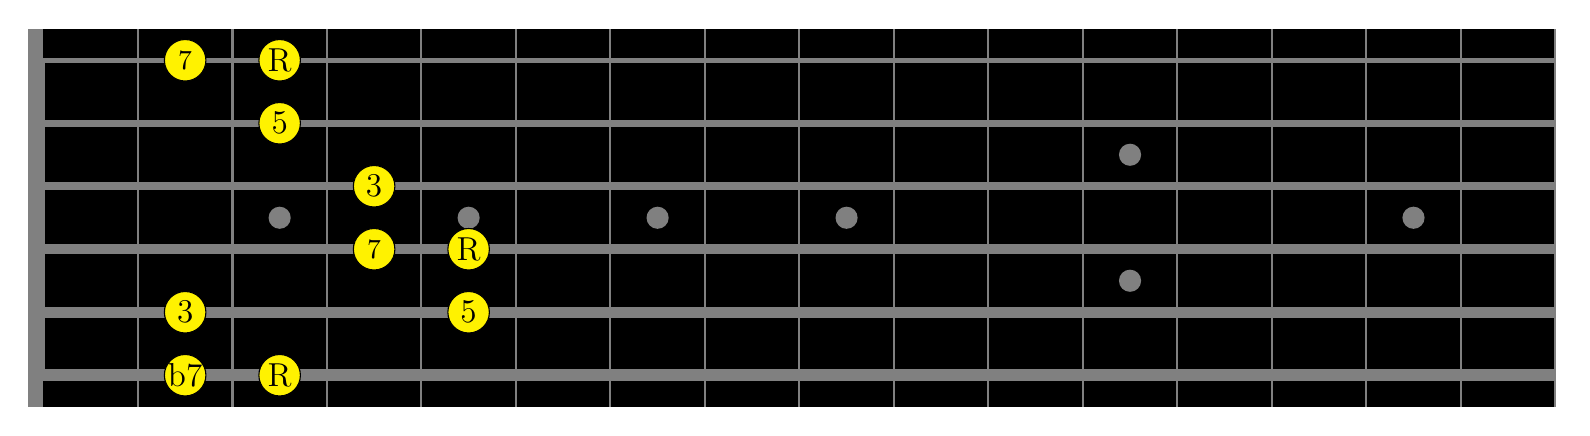
\begin{tikzpicture}[scale=1]
	\def \h{0.8}
	\def \fret{1.2} % 1.6
	\def \L{ 16*\fret }	
	\def \dot_size{4pt}
	\def \circ_size{15pt}
	
	\fill[black, line width=2] (0.0,-0.4) rectangle (16*\fret,4.4);
	\fill[black!50!white, line width=2] (-0.2,-0.4) rectangle (0,4.4);
	
	% Strings
	\draw[color=black!50!white, line width=2.0]  (-0.1, 5*\h) -- (\L,5*\h); % E
	\draw[color=black!50!white, line width=2.5]  (-0.1, 4*\h) -- (\L,4*\h); % B
	\draw[color=black!50!white, line width=3.0]  (-0.1, 3*\h) -- (\L,3*\h); % G
	\draw[color=black!50!white, line width=3.5]  (-0.1, 2*\h) -- (\L,2*\h); % D
	\draw[color=black!50!white, line width=4.0]  (-0.1, 1*\h) -- (\L,1*\h); % A
	\draw[color=black!50!white, line width=4.5]  (-0.1, 0*\h) -- (\L,0*\h); % E
	
	% Frets 0
	\draw[color=black!50!white, thick]  (-0.1, 0) -- (-0.1,5*\h); 
	\draw[color=black!50!white, thick]  (0, 0)   -- (0,5*\h); 
	
	% Fret 1-15
	\draw[color=black!50!white, thick]  (\fret,   -0.4)   -- (\fret,4.4);   
	\draw[color=black!50!white, thick]  (2*\fret, -0.4) -- (2*\fret,4.4); 
	\draw[color=black!50!white, thick]  (3*\fret, -0.4) -- (3*\fret,4.4); 
	\draw[color=black!50!white, thick]  (4*\fret, -0.4) -- (4*\fret,4.4); 
	\draw[color=black!50!white, thick]  (5*\fret, -0.4) -- (5*\fret,4.4); 
	\draw[color=black!50!white, thick]  (6*\fret, -0.4) -- (6*\fret,4.4); 
	\draw[color=black!50!white, thick]  (7*\fret, -0.4) -- (7*\fret,4.4); 
	\draw[color=black!50!white, thick]  (8*\fret, -0.4) -- (8*\fret,4.4); 
	\draw[color=black!50!white, thick]  (9*\fret, -0.4) -- (9*\fret,4.4); 
	\draw[color=black!50!white, thick]  (10*\fret, -0.4) -- (10*\fret,4.4); 
	\draw[color=black!50!white, thick]  (11*\fret, -0.4) -- (11*\fret,4.4); 
	\draw[color=black!50!white, thick]  (12*\fret, -0.4) -- (12*\fret,4.4); 
	\draw[color=black!50!white, thick]  (13*\fret, -0.4) -- (13*\fret,4.4); 
	\draw[color=black!50!white, thick]  (14*\fret, -0.4) -- (14*\fret,4.4); 
	\draw[color=black!50!white, thick]  (15*\fret, -0.4) -- (15*\fret,4.4); 
	\draw[color=black!50!white, thick]  (16*\fret, -0.4) -- (16*\fret,4.4); 
	%\draw[color=black!50!white, thick]  (17*\fret, -0.4) -- (17*\fret,4.4); 
	%\draw[color=black!50!white, thick]  (18*\fret, -0.4) -- (18*\fret,4.4); 
	%\draw[color=black!50!white, thick]  (19*\fret, -0.4) -- (19*\fret,4.4); 
	%\draw[color=black!50!white, thick]  (20*\fret, -0.4) -- (20*\fret,4.4); 
	
	% Dots
	\fill[black!50!white] (2.5*\fret,2.5*\h) circle (\dot_size); % fret 3
	\fill[black!50!white] (4.5*\fret,2.5*\h) circle (\dot_size); % fret 5
	\fill[black!50!white] (6.5*\fret,2.5*\h) circle (\dot_size); % fret 7
	\fill[black!50!white] (8.5*\fret,2.5*\h) circle (\dot_size); % fret 9
	\fill[black!50!white] (11.5*\fret,1.5*\h) circle (\dot_size); % fret 12
	\fill[black!50!white] (11.5*\fret,3.5*\h) circle (\dot_size); % fret 12
	\fill[black!50!white] (14.5*\fret,2.5*\h) circle (\dot_size); % fret 15
	%\fill[black!50!white] (16.5*\fret,2.5*\h) circle (\dot_size); % fret 17
	%\fill[black!50!white] (18.5*\fret,2.5*\h) circle (\dot_size); % fret 19

	
	% Arpege (position E)
	\node[dot=\circ_size, fill=yellow,draw] at (1.5*\fret,0) {{\large b7}};
	\node[dot=\circ_size, fill=yellow,draw] at (2.5*\fret,0) {{\large R}};
	\node[dot=\circ_size, fill=yellow,draw] at (1.5*\fret,1*\h) {{\large 3}};
	%\node[dot=\circ_size, fill=yellow,draw] at (1.5*\fret,1*\h) {{\large 3}};
	\node[dot=\circ_size, fill=yellow,draw] at (4.5*\fret,1*\h) {{\large 5}};
	\node[dot=\circ_size, fill=yellow,draw] at (3.5*\fret,2*\h) {{\normalsize 7}};
	\node[dot=\circ_size, fill=yellow,draw] at (4.5*\fret,2*\h) {{\large R}};
	\node[dot=\circ_size, fill=yellow,draw] at (3.5*\fret,3*\h) {{\large 3}};
	\node[dot=\circ_size, fill=yellow,draw] at (2.5*\fret,4*\h) {{\large 5}};
	\node[dot=\circ_size, fill=yellow,draw] at (1.5*\fret,5*\h) {{\normalsize 7}};
	\node[dot=\circ_size, fill=yellow,draw] at (2.5*\fret,5*\h) {{\large R}};
	
%	% Arpege (position D-C)
%	\node[dot=\circ_size, fill=white,draw] at (8.5*\fret,1*\h) {{\normalsize 7}};
%	\node[dot=\circ_size, fill=yellow!50!red!65!white,draw] at (9.5*\fret,1*\h) {{\large R}};
%	\node[dot=\circ_size, fill=yellow!50!red!30!white,draw] at (8.5*\fret,2*\h) {{\large 3}};
%	\node[dot=\circ_size, fill=yellow!50!red!30!white,draw] at (6.5*\fret,3*\h) {{\large 5}};
%	\node[dot=\circ_size, fill=white,draw] at (6.5*\fret,4*\h) {{\normalsize M7}};
%	\node[dot=\circ_size, fill=yellow!50!red!30!white,draw] at (7.5*\fret,4*\h) {{\large R}};
%	\node[dot=\circ_size, fill=yellow!100!red!50!white,draw] at (6.5*\fret,5*\h) {{\large 3}};
%	\node[dot=\circ_size, fill=yellow!50!red!65!white,draw] at (9.5*\fret,5*\h) {{\large 5}};
	
	% Arpege (position A)
%	\node[dot=\circ_size, fill=yellow!50!red!80!white,draw] at (13.5*\fret,1*\h) {{\large 3}};
%	\node[dot=\circ_size, fill=yellow!50!red!80!white,draw] at (11.5*\fret,2*\h) {{\large 5}};
%	\node[dot=\circ_size, fill=white,draw] at (10.5*\fret,3*\h) {{\normalsize M7}};
%	\node[dot=\circ_size, fill=yellow!50!red!80!white,draw] at (11.5*\fret,3*\h) {{\large R}};
%	\node[dot=\circ_size, fill=yellow!50!red!80!white,draw] at (11.5*\fret,4*\h) {{\large 3}};
%	\node[dot=\circ_size, fill=white,draw] at (13.5*\fret,5*\h) {{\normalsize M7}};
%	\node[dot=\circ_size, fill=yellow!50!red!80!white,draw] at (14.5*\fret,5*\h) {{\large R}};

%	% Annotation
%	\draw[black,anchor=west] (-3cm,2cm) node { {\Huge $\Delta$7 } };
	
\end{tikzpicture}
%\end{document}




}
	\hspace*{-0cm}
	\scalebox{0.52}{\input{figures/arpeges/m7b5/m7b5_pos1.tex}}

	\hspace*{-4.2cm}
	\scalebox{0.52}{\input{figures/arpeges/maj7/maj7_pos2.tex}}
	\hspace*{-0cm}
	\scalebox{0.52}{\input{figures/arpeges/m7b5/m7b5_pos2.tex}}

	\hspace*{-4.2cm}
	\scalebox{0.52}{\input{figures/arpeges/maj7/maj7_pos3.tex}}
	\hspace*{-0cm}
	\scalebox{0.52}{\input{figures/arpeges/m7b5/m7b5_pos3.tex}}

	\hspace*{-4.2cm}
	\scalebox{0.52}{\input{figures/arpeges/maj7/maj7_pos4.tex}}
	\hspace*{-0cm}
	\scalebox{0.52}{\input{figures/arpeges/m7b5/m7b5_pos4.tex}}

	\hspace*{-4.2cm}
	\scalebox{0.52}{\input{figures/arpeges/maj7/maj7_pos5.tex}}
	\hspace*{-0cm}
	\scalebox{0.52}{\input{figures/arpeges/m7b5/m7b5_pos5.tex}}

	\caption{(left) maj7 arpeggio. (right) m7b5 arpeggio}
	\label{fig:arpeggio}
\end{table}



%%%%%%%%%%%%%%%%%%%%%%%%%%%%%%%%%%%%%%%%%%%%%%%%%%%%%%%%%%%%%%%%%%
\newpage
\section{Modes}

\begin{itemize}
	\item Ionian (Joy), dorian(Jazz), phrygian(flamenco,doom), lydian (floaty,mystery) (ex: E.T., Jurassic Park, Back to the Future), mixo(blues)(ex: AC/DC), aeolian(sad)(ex: Losing my Religion), locrian(tension)(ex:Bjork Army of Me)
\end{itemize}

%%%%%%%%%%%%%%%%%%%%%%%%%%%%%%%%%%%%%%%%%%%%%%%%%%%%%%%%%%%%%%%%%%
\newpage
\section{Transposition}

https://www.youtube.com/watch?v=Vxac3hHrxg8

%%%%%%%%%%%%%%%%%%%%%%%%%%%%%%%%%%%%%%%%%%%%%%%%%%%%%%%%%%%%%%%%%%
\newpage
\section{Composition variation (Shred Master Scott)}

\begin{itemize}
	\item Pedal tone
	\item Inversion
	\item Voice leading
\end{itemize}

%\newpage
%\bibliographystyle{plain}
%\bibliography{/home/jh/Documents/library.bib}

\end{document}
